% preview.tex -- compiles all draft figures onto one multi-page PDF for
% review. Reuses the paper's own preamble (colors, macros) so what you see
% here matches how these figures would actually render if copied into
% main.tex or appendix.tex. Not itself part of the paper.
%
%   cd figure_drafts && pdflatex preview.tex
%
% (untested in this environment -- no pdflatex was available when authored;
% check for overlaps/overfull boxes before trusting the layout.)

\documentclass[10pt,letterpaper]{article}
\usepackage[margin=1.2cm]{geometry}
\usepackage{xcolor}
% ============================================================================
% PhysWeep preamble (shared by main.tex and appendix.tex).
% wacv.sty already provides: times, xcolor (dvipsnames), graphicx, amsmath,
% amssymb, booktabs, natbib[numbers,sort&compress], caption, subcaption, url,
% enumitem[shortlabels,inline]. Do NOT reload any of those here.
% ============================================================================

\usepackage{amsthm}
\usepackage{array}
\usepackage{tikz}
\usetikzlibrary{arrows.meta,positioning,calc,backgrounds,fit,patterns}
\usepackage{algorithm}
\usepackage{algpseudocode}
\usepackage{pifont}

% --- red-flag macros: every item the authors must supply before submission.
% Search the source for "MISSING" / "VERIFY" to find them all; they render in
% red in the PDF so none can ship unnoticed.
\newcommand{\MISSING}[1]{\textcolor{red}{[MISSING: #1]}}
\newcommand{\VERIFYFLAG}[1]{\textcolor{red}{[VERIFY: #1]}}

\newcommand{\cmark}{\textcolor{green!55!black}{\ding{51}}}
\newcommand{\xmark}{\textcolor{red!70!black}{\ding{55}}}

% Keep theorem statements from orphaning their header across a column break.
% Without this, a Proposition whose header lands exactly at a column boundary
% is shipped out above the running header and bleeds off the page edge
% (observed as "Overfull \hbox ... while \output is active").
\usepackage{needspace}
\usepackage{colortbl}   % \cellcolor for the coverage heat map
\usepackage{multirow}

% --- coverage heat map -----------------------------------------------------
% Single-hue sequential ramp so the table stays legible in grayscale, which
% top venues still print in. Zero is rendered in gray rather than white so a
% measured zero is visually distinct from an empty cell.
\definecolor{trkhi}{RGB}{31,102,160}
\newcommand{\tzero}{\cellcolor{black!8}\textcolor{black!55}{$0$}}
\newcommand{\tk}[2]{\cellcolor{trkhi!#1}$#2$}
\newcommand{\tkb}[2]{\cellcolor{trkhi!#1}$\mathbf{#2}$}
% compact in-table placeholder for a value the authors must still compute;
% the matching \MISSING{} lives in the caption so it reaches the red-flag list
\newcommand{\tbd}{\cellcolor{red!12}\textcolor{red!80!black}{\textbf{?}}}

% Non-floating tables in a plain center environment inherit \topsep and
% \parskip above and below, which costs roughly 25pt per table. This wrapper
% keeps the centring and drops the padding.
\newenvironment{tightcenter}
  {\setlength{\topsep}{1pt}\setlength{\partopsep}{0pt}%
   \setlength{\parskip}{0pt}\par\centering}
  {\par\addvspace{2pt}}
\newtheorem{proposition}{Proposition}
% Unnumbered form for restating a main-paper result in the supplementary, so
% the supplementary does not assign it a second, different number.
\newtheorem*{propositionstar}{Proposition}
\newtheorem{definition}{Definition}
\newtheorem{remark}{Remark}
\newtheorem{assumption}{Assumption}

\newcommand{\PRE}{\ensuremath{\mathrm{PRE}}}
\newcommand{\PRI}{\ensuremath{\mathrm{PRI}}}
\newcommand{\CBI}{\ensuremath{\mathrm{CBI}}}
\newcommand{\EG}{\ensuremath{\mathrm{EG}}}
\newcommand{\thetah}{\ensuremath{\hat{\theta}}}

% --- line-number overlap fix (applies only if wacv.sty loaded lineno)
\makeatletter
\AtBeginDocument{\@ifpackageloaded{lineno}{%
  \setlength{\linenumbersep}{6pt}%
  \renewcommand\linenumberfont{\normalfont\scriptsize\color{gray}}%
  % Consecutive line numbers can stack on top of each other where a
  % display or a centered block compresses baseline spacing. Setting a
  % minimum inter-number distance stops that without touching text layout.
  \setlength{\linenumberwidth}{18pt}%
  \leftlinenumbers}{}}
\makeatother

\usetikzlibrary{decorations.pathmorphing}  % coil, for the spring-mass sketch
\usepackage{caption}

\title{PhysWeep -- draft figures (not yet in main.tex)}
\author{}
\date{}

\begin{document}
\maketitle
\tableofcontents

\clearpage
\section{Pipeline diagram (creative/explanatory)}
\begin{figure}[h]\centering
\resizebox{\textwidth}{!}{% fig_pipeline.tex -- the PhysWeep audit pipeline as a flow diagram.
% Draft only, not yet wired into main.tex. Standalone-compilable via
% preview.tex or wrapped in its own \documentclass{standalone}.
%
% Shows: theta (ground truth) -> deterministic renderer -> conditioning
% frames -> frozen generator -> generated clip -> tracker+fitter ->
% theta_hat -> metrics (PRE/EG/PRI/CBI/SDI). This is the "how it works"
% figure a reader wants before the Metrics section's equations.

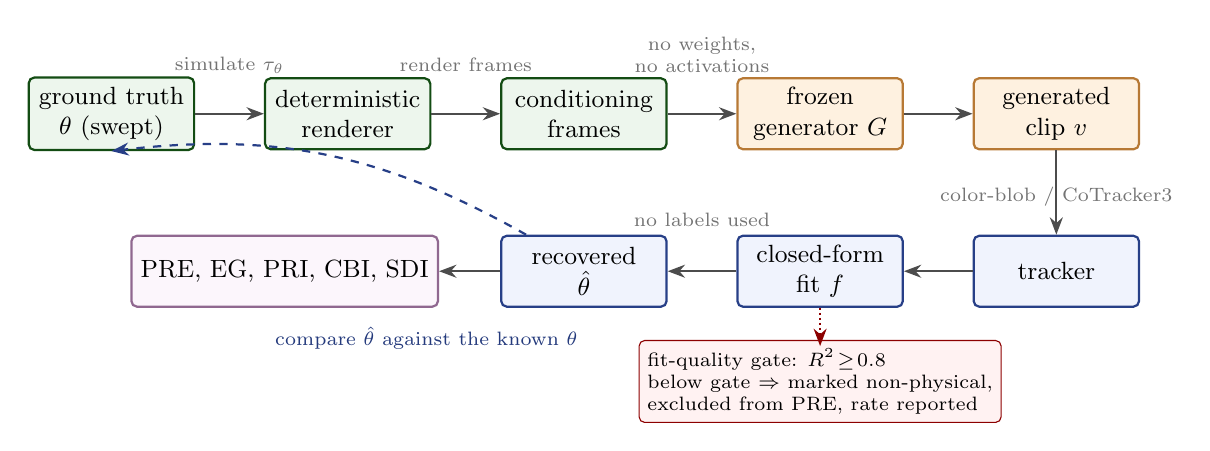
\begin{tikzpicture}[
  font=\small,
  box/.style={draw=black!70, rounded corners=2pt, minimum height=0.9cm,
              minimum width=2.1cm, align=center, fill=white, line width=0.8pt},
  known/.style={box, fill=ForestGreen!8, draw=ForestGreen!55!black},
  frozen/.style={box, fill=BurntOrange!10, draw=BurntOrange!70!black},
  measure/.style={box, fill=RoyalBlue!8, draw=RoyalBlue!60!black},
  metric/.style={box, fill=Plum!10, draw=Plum!65!black, minimum width=2.6cm},
  arr/.style={-{Stealth[length=2.2mm]}, thick, black!70},
  lbl/.style={font=\scriptsize, black!55, align=center}
]

% ---- top row: the generative half ----
\node[known] (theta) at (0,0) {ground truth\\$\theta$ (swept)};
\node[known] (render) at (3.0,0) {deterministic\\renderer};
\node[known] (cond) at (6.0,0) {conditioning\\frames};
\node[frozen] (gen) at (9.0,0) {frozen\\generator $G$};
\node[frozen] (clip) at (12.0,0) {generated\\clip $v$};

\draw[arr] (theta) -- (render);
\draw[arr] (render) -- (cond);
\draw[arr] (cond) -- (gen);
\draw[arr] (gen) -- (clip);

\node[lbl] at (1.5,0.62) {simulate $\tau_\theta$};
\node[lbl] at (4.5,0.62) {render frames};
\node[lbl,align=center] at (7.5,0.75) {no weights,\\no activations};

% ---- bottom row: the measurement half, running back left ----
\node[measure] (track) at (12.0,-2.0) {tracker};
\node[measure] (fit) at (9.0,-2.0) {closed-form\\fit $f$};
\node[measure] (thetahat) at (6.0,-2.0) {recovered\\$\thetah$};
\node[metric] (metrics) at (2.2,-2.0) {\PRE, \EG, \PRI, \CBI, SDI};

\draw[arr] (clip) -- (track);
\draw[arr] (track) -- (fit);
\draw[arr] (fit) -- (thetahat);
\draw[arr] (thetahat) -- (metrics);

\node[lbl] at (12.0,-1.05) {color-blob / CoTracker3};
\node[lbl] at (7.5,-1.35) {no labels used};

% ---- the comparison arrow that closes the loop: theta vs theta_hat ----
\draw[arr, RoyalBlue!60!black, dashed] (thetahat) to[bend right=18] (theta.south);
\node[lbl, RoyalBlue!55!black] at (4.0,-2.85) {compare $\thetah$ against the known $\theta$};

% ---- gate annotation ----
\node[draw=red!55!black, fill=red!5, rounded corners=2pt, font=\scriptsize,
      align=left, inner sep=3pt] at (9.0,-3.4)
  {fit-quality gate: $R^2 \!\ge\! 0.8$\\
   below gate $\Rightarrow$ marked non-physical,\\
   excluded from \PRE, rate reported};
\draw[arr, red!55!black, densely dotted] (fit.south) -- (9.0,-2.95);

\end{tikzpicture}
}
\caption{The full audit pipeline: ground truth $\theta$ through the
deterministic renderer, the frozen generator, and back through the
tracker/fitter to $\hat\theta$ and the metrics. Candidate for the
Suite/Pipeline section (Section~4 of \texttt{main.tex}).}
\end{figure}

\clearpage
\section{Dataset examples}
\begin{figure}[h]\centering
\resizebox{0.85\textwidth}{!}{% fig_dataset_examples.tex -- dataset examples: one schematic frame-strip
% per system, showing what a conditioning sequence + swept theta produces.
% Draft only. Real grids/units taken from main.tex's Table (tab:suite).
%
% Each row: a short strip of 4 schematic frames (ball/disk on plain
% background against ground/pivot/wall as appropriate) at increasing time,
% with theta and its true grid values annotated. This is meant to show a
% reader concretely what "the PhysWeep suite" renders, since the paper's
% own suite table (tab:suite) is text-only.
%
% REQUIRES: \usetikzlibrary{decorations.pathmorphing} (for the spring
% coil in the spring-mass row) -- not loaded by main.tex's preamble.tex,
% add it if copying this figure in.

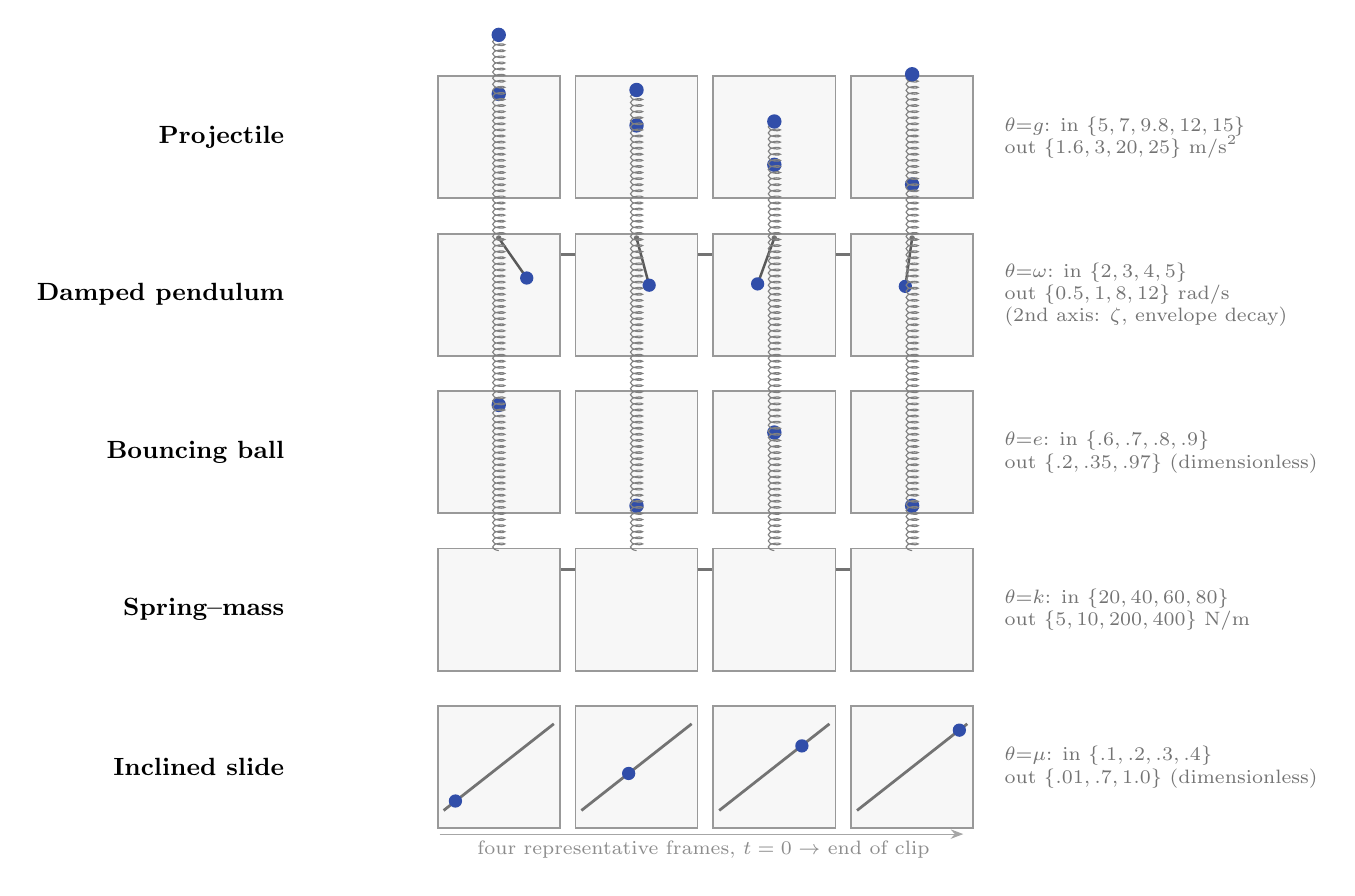
\begin{tikzpicture}[
  font=\small,
  framebox/.style={draw=black!40, fill=black!3, minimum width=1.55cm,
                    minimum height=1.55cm, line width=0.6pt},
  disk/.style={fill=RoyalBlue!75!black, draw=none},
  ground/.style={black!55, line width=1.0pt},
  rowlbl/.style={font=\bfseries\small, anchor=east},
  gridlbl/.style={font=\scriptsize, black!55, anchor=west, align=left}
]

% column x-centers for the 4-frame strip
\def\colx{0,1.75,3.5,5.25}
\def\rowlabelx{-2.6}
\def\stripstartx{-1.0}

% ============ ROW 1: projectile ============
\node[rowlbl] at (\rowlabelx,0) {Projectile};
\foreach \i/\x in {1/0,2/1.75,3/3.5,4/5.25}{
  \node[framebox] (p\i) at (\x,0) {};
}
\draw[ground] ([yshift=-0.7cm]p1.south west) -- ([yshift=-0.7cm]p4.south east);
% falling arc across 4 frames, y decreasing then bottoming out
\fill[disk] (p1.center)+(0,0.55) circle (2.6pt);
\fill[disk] (p2.center)+(0,0.15) circle (2.6pt);
\fill[disk] (p3.center)+(0,-0.35) circle (2.6pt);
\fill[disk] (p4.center)+(0,-0.6) circle (2.6pt);
\node[gridlbl] at (6.3,0) {$\theta{=}g$: in $\{5,7,9.8,12,15\}$\\out $\{1.6,3,20,25\}$ m/s$^2$};

% ============ ROW 2: damped pendulum ============
\node[rowlbl] at (\rowlabelx,-2.0) {Damped pendulum};
\foreach \i/\x in {1/0,2/1.75,3/3.5,4/5.25}{
  \node[framebox] (d\i) at (\x,-2.0) {};
}
\foreach \i/\x/\ang in {1/0/35,2/1.75/15,3/3.5/-20,4/5.25/-8}{
  \fill[black!55] ([yshift=0.72cm]d\i.center) circle (1.0pt);
  \draw[black!65,line width=0.9pt] ([yshift=0.72cm]d\i.center) -- ++({-90+\ang}:0.62cm);
  \fill[disk] ([yshift=0.72cm]d\i.center) ++({-90+\ang}:0.62cm) circle (2.4pt);
}
\node[gridlbl] at (6.3,-2.0) {$\theta{=}\omega$: in $\{2,3,4,5\}$\\out $\{0.5,1,8,12\}$ rad/s\\(2nd axis: $\zeta$, envelope decay)};

% ============ ROW 3: bouncing ball ============
\node[rowlbl] at (\rowlabelx,-4.0) {Bouncing ball};
\foreach \i/\x in {1/0,2/1.75,3/3.5,4/5.25}{
  \node[framebox] (b\i) at (\x,-4.0) {};
}
\draw[ground] ([yshift=-0.7cm]b1.south west) -- ([yshift=-0.7cm]b4.south east);
\fill[disk] (b1.center)+(0,0.6) circle (2.6pt);
\fill[disk] (b2.center)+(0,-0.68) circle (2.6pt);
\fill[disk] (b3.center)+(0,0.25) circle (2.6pt);
\fill[disk] (b4.center)+(0,-0.68) circle (2.6pt);
\node[gridlbl] at (6.3,-4.0) {$\theta{=}e$: in $\{.6,.7,.8,.9\}$\\out $\{.2,.35,.97\}$ (dimensionless)};

% ============ ROW 4: spring-mass ============
\node[rowlbl] at (\rowlabelx,-6.0) {Spring--mass};
\foreach \i/\x in {1/0,2/1.75,3/3.5,4/5.25}{
  \node[framebox] (s\i) at (\x,-6.0) {};
}
\foreach \i/\x/\yy in {1/0/0.55,2/1.75/-0.15,3/3.5/-0.55,4/5.25/0.05}{
  \draw[black!50,decorate,decoration={coil,aspect=0.35,segment length=2.2pt,amplitude=2.2pt}]
    ([yshift=0.75cm]s\i.center) -- ([yshift=0.75cm]s\i.center |- {0,\yy});
  \fill[disk] ([yshift=0.75cm]s\i.center |- {0,\yy}) circle (2.6pt);
}
\node[gridlbl] at (6.3,-6.0) {$\theta{=}k$: in $\{20,40,60,80\}$\\out $\{5,10,200,400\}$ N/m};

% ============ ROW 5: inclined slide ============
\node[rowlbl] at (\rowlabelx,-8.0) {Inclined slide};
\foreach \i/\x in {1/0,2/1.75,3/3.5,4/5.25}{
  \node[framebox] (i\i) at (\x,-8.0) {};
}
\foreach \i in {1,2,3,4}{
  \draw[black!55,line width=1.0pt] ([xshift=-0.7cm,yshift=-0.55cm]i\i.center) -- ([xshift=0.7cm,yshift=0.55cm]i\i.center);
}
\fill[disk] ([xshift=-0.55cm,yshift=-0.43cm]i1.center) circle (2.4pt);
\fill[disk] ([xshift=-0.1cm,yshift=-0.08cm]i2.center) circle (2.4pt);
\fill[disk] ([xshift=0.35cm,yshift=0.27cm]i3.center) circle (2.4pt);
\fill[disk] ([xshift=0.6cm,yshift=0.47cm]i4.center) circle (2.4pt);
\node[gridlbl] at (6.3,-8.0) {$\theta{=}\mu$: in $\{.1,.2,.3,.4\}$\\out $\{.01,.7,1.0\}$ (dimensionless)};

% time axis label under the whole strip
\node[font=\scriptsize,black!45] at (2.6,-9.05) {four representative frames, $t=0 \to$ end of clip};
\draw[-{Stealth[length=1.6mm]},black!35] (-0.75,-8.85) -- (5.9,-8.85);

\end{tikzpicture}
}
\caption{Schematic conditioning-sequence examples for all five systems
(six sweep axes). Candidate for Section~4 (Suite), as a visual companion
to \texttt{tab:suite}.}
\end{figure}

\clearpage
\section{Results example: full seed scatter}
\begin{figure}[h]\centering
\resizebox{0.85\textwidth}{!}{% fig_seed_scatter.tex -- results example: ALL 5 gated seeds for the
% CogVideoX/projectile in-range grid (Figure 1 panel (a) only shows 2).
% Draft only. Data below is the real per-clip gated (R^2>=0.8) g_hat from
% results/e0_pilot_cogvideox.json, reproduced exactly (see CLAUDE.md
% Section 5, "E0 (CogVideoX-5B-I2V)"). Magnitudes plotted (sign flipped),
% matching Figure 1's own convention.
%
% seed 0: (5,11.41) (7,11.39) (9.8,11.40) (12,11.46) (15,11.41)
% seed 1: (5,11.37) (7,11.41) (9.8,11.34) (12,11.79) (15,11.44)
% seed 2: (5,13.33)                                              [n=1, not a cluster]
% seed 3: (5,11.83)        (9.8,11.98) (12,10.71) (15,10.45)
% seed 4: (5,7.31) (7,7.00) (9.8,6.80) (12,7.06) (15,15,7.22)

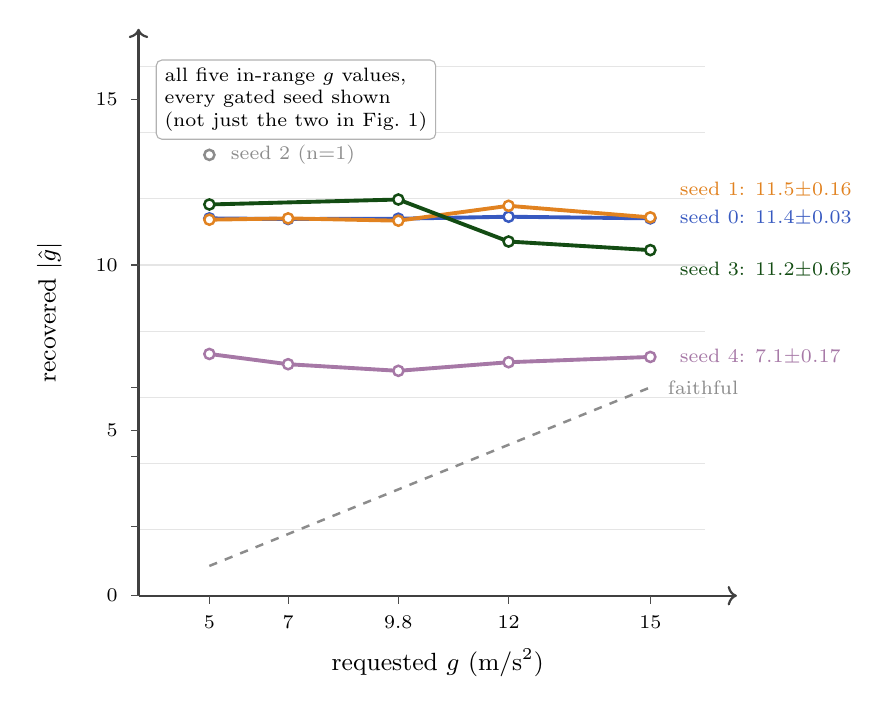
\begin{tikzpicture}[
  font=\small,
  ax/.style={->,thick,black!75},
  gridln/.style={black!10,line width=0.4pt},
  ideal/.style={dashed,black!45,line width=0.9pt},
  s0/.style={RoyalBlue!85!black},
  s1/.style={BurntOrange!90!black},
  s2/.style={black!45},
  s3/.style={ForestGreen!55!black},
  s4/.style={Plum!75!black},
  mk/.style={circle,inner sep=1.3pt,draw,line width=0.9pt,fill=white}
]

\foreach \y in {2,4,...,16}{\draw[gridln] (0,\y*0.42) -- (7.2,\y*0.42);}
\draw[ax] (0,0) -- (7.6,0);
\draw[ax] (0,0) -- (0,7.2);
\foreach \g/\x in {5/0.9,7/1.9,9.8/3.3,12/4.7,15/6.5}
  {\draw[black!70] (\x,0) -- (\x,-0.1); \node[font=\scriptsize,anchor=north] at (\x,-0.14) {\g};}
\foreach \v/\y in {0/0,5/2.1,10/4.2,15/6.3}
  {\draw[black!70] (0,\y*0.42*1) -- (-0.1,\y*0.42*1); \node[font=\scriptsize,anchor=east] at (-0.14,\y*0.42*1) {};}
\foreach \v in {0,5,10,15}
  {\draw[black!70] (0,\v*0.42) -- (-0.1,\v*0.42); \node[font=\scriptsize,anchor=east] at (-0.14,\v*0.42) {\v};}
\node[font=\small,anchor=north] at (3.8,-0.55) {requested $g$ (m/s$^2$)};
\node[font=\small,rotate=90,anchor=south] at (-0.85,3.6) {recovered $|\hat g|$};

% identity / faithful reference
\draw[ideal] (0.9,0.9*0.42) -- (6.5,6.3*0.42);
\node[black!45,font=\scriptsize,anchor=west] at (6.6,6.3*0.42) {faithful};

% seed 0
\draw[s0,line width=1.4pt] (0.9,11.41*0.42) -- (1.9,11.39*0.42) -- (3.3,11.40*0.42) -- (4.7,11.46*0.42) -- (6.5,11.41*0.42);
\foreach \x/\v in {0.9/11.41,1.9/11.39,3.3/11.40,4.7/11.46,6.5/11.41}{\node[mk,draw=RoyalBlue!85!black] at (\x,\v*0.42) {};}

% seed 1
\draw[s1,line width=1.4pt] (0.9,11.37*0.42) -- (1.9,11.41*0.42) -- (3.3,11.34*0.42) -- (4.7,11.79*0.42) -- (6.5,11.44*0.42);
\foreach \x/\v in {0.9/11.37,1.9/11.41,3.3/11.34,4.7/11.79,6.5/11.44}{\node[mk,draw=BurntOrange!90!black] at (\x,\v*0.42) {};}

% seed 3 (only 4 gated points)
\draw[s3,line width=1.4pt] (0.9,11.83*0.42) -- (3.3,11.98*0.42) -- (4.7,10.71*0.42) -- (6.5,10.45*0.42);
\foreach \x/\v in {0.9/11.83,3.3/11.98,4.7/10.71,6.5/10.45}{\node[mk,draw=ForestGreen!55!black] at (\x,\v*0.42) {};}

% seed 4
\draw[s4,line width=1.4pt] (0.9,7.31*0.42) -- (1.9,7.00*0.42) -- (3.3,6.80*0.42) -- (4.7,7.06*0.42) -- (6.5,7.22*0.42);
\foreach \x/\v in {0.9/7.31,1.9/7.00,3.3/6.80,4.7/7.06,6.5/7.22}{\node[mk,draw=Plum!75!black] at (\x,\v*0.42) {};}

% seed 2 (only 1 gated point, shown as a lone marker, not a cluster)
\node[mk,draw=black!45] at (0.9,13.33*0.42) {};
\node[font=\scriptsize,black!45,anchor=west] at (1.05,13.33*0.42) {seed 2 (n=1)};

% right-hand legend
\node[s0,font=\scriptsize,anchor=west] at (6.75,11.41*0.42) {seed 0: $11.4{\pm}0.03$};
\node[s1,font=\scriptsize,anchor=west] at (6.75,11.44*0.42+0.35) {seed 1: $11.5{\pm}0.16$};
\node[s3,font=\scriptsize,anchor=west] at (6.75,10.45*0.42-0.25) {seed 3: $11.2{\pm}0.65$};
\node[s4,font=\scriptsize,anchor=west] at (6.75,7.22*0.42) {seed 4: $7.1{\pm}0.17$};

\node[draw=black!30,fill=white,rounded corners=2pt,inner sep=3pt,font=\scriptsize,align=left]
  at (2.0,6.3) {all five in-range $g$ values,\\every gated seed shown\\(not just the two in Fig.~1)};

\end{tikzpicture}
}
\caption{All five gated seeds for CogVideoX/projectile in-range (Figure~1
panel~a in \texttt{main.tex} shows only two). Candidate as a supplementary
figure (Sec.~S4) or a Results-section inset.}
\end{figure}

\clearpage
\section{Mechanism shapes (creative/explanatory)}
\begin{figure}[h]\centering
\resizebox{\textwidth}{!}{% fig_mechanism_shapes.tex -- creative/explanatory: a clean, standalone
% redraw of "which response shape is it" (same geometry as Fig.~1 panel c,
% but bigger, on its own, with each of the THREE shapes drawn separately
% so a reader can absorb one at a time rather than overlaid). Good for the
% Metrics or Problem section as a companion to Eq.~(pri)/(cbi).
% Draft only, not wired into main.tex.

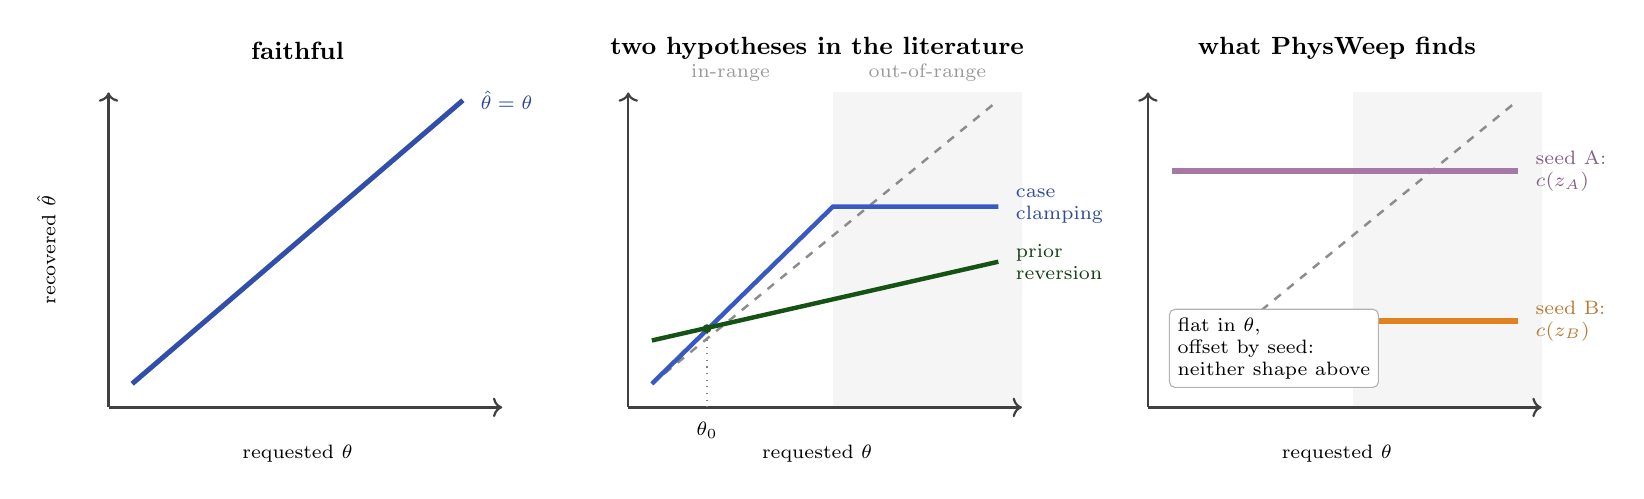
\begin{tikzpicture}[
  font=\small,
  ax/.style={->,thick,black!75},
  ideal/.style={dashed,black!45,line width=0.9pt},
  panelbg/.style={fill=black!4},
]

% ---------- PANEL 1: faithful ----------
\begin{scope}
  \node[anchor=south,font=\bfseries\small] at (2.4,4.3) {faithful};
  \draw[ax] (0,0) -- (5.0,0);
  \draw[ax] (0,0) -- (0,4.0);
  \node[font=\scriptsize,anchor=north] at (2.4,-0.35) {requested $\theta$};
  \node[font=\scriptsize,rotate=90,anchor=south] at (-0.55,2.0) {recovered $\hat\theta$};
  \draw[RoyalBlue!75!black,line width=1.8pt] (0.3,0.3) -- (4.5,3.9);
  \node[RoyalBlue!65!black,font=\scriptsize,anchor=west] at (4.6,3.9) {$\hat\theta=\theta$};
\end{scope}

% ---------- PANEL 2: the two prior hypotheses ----------
\begin{scope}[shift={(6.6,0)}]
  \node[anchor=south,font=\bfseries\small] at (2.4,4.3) {two hypotheses in the literature};
  \fill[panelbg] (2.6,0) rectangle (5.0,4.0);
  \draw[ax] (0,0) -- (5.0,0);
  \draw[ax] (0,0) -- (0,4.0);
  \node[black!40,font=\scriptsize,anchor=south] at (1.3,4.02) {in-range};
  \node[black!40,font=\scriptsize,anchor=south] at (3.8,4.02) {out-of-range};
  \node[font=\scriptsize,anchor=north] at (2.4,-0.35) {requested $\theta$};
  \draw[ideal] (0.3,0.3) -- (4.7,3.9);
  % case clamping: follows identity then flat
  \draw[RoyalBlue!85!black,line width=1.6pt] (0.3,0.3) -- (2.6,2.55) -- (4.7,2.55);
  \node[RoyalBlue!70!black,font=\scriptsize,anchor=west,align=left] at (4.8,2.55)
    {case\\clamping};
  % prior reversion: shallow line crossing identity at theta_0
  \draw[ForestGreen!60!black,line width=1.6pt] (0.3,0.85) -- (4.7,1.85);
  \fill[ForestGreen!60!black] (1.0,1.0) circle (1.6pt);
  \node[ForestGreen!45!black,font=\scriptsize,anchor=west,align=left] at (4.8,1.85)
    {prior\\reversion};
  \node[font=\scriptsize,anchor=north] at (1.0,-0.06) {$\theta_0$};
  \draw[black!50,dotted] (1.0,0) -- (1.0,1.0);
\end{scope}

% ---------- PANEL 3: what we actually find ----------
\begin{scope}[shift={(13.2,0)}]
  \node[anchor=south,font=\bfseries\small] at (2.4,4.3) {what PhysWeep finds};
  \fill[panelbg] (2.6,0) rectangle (5.0,4.0);
  \draw[ax] (0,0) -- (5.0,0);
  \draw[ax] (0,0) -- (0,4.0);
  \node[font=\scriptsize,anchor=north] at (2.4,-0.35) {requested $\theta$};
  \draw[ideal] (0.3,0.3) -- (4.7,3.9);
  % two flat, seed-conditional levels
  \draw[Plum!75!black,line width=2.0pt] (0.3,3.0) -- (4.7,3.0);
  \draw[BurntOrange!90!black,line width=2.0pt] (0.3,1.1) -- (4.7,1.1);
  \node[Plum!60!black,font=\scriptsize,anchor=west,align=left] at (4.8,3.0)
    {seed A:\\$c(z_A)$};
  \node[BurntOrange!70!black,font=\scriptsize,anchor=west,align=left] at (4.8,1.1)
    {seed B:\\$c(z_B)$};
  \node[draw=black!30,fill=white,rounded corners=2pt,inner sep=3pt,
        font=\scriptsize,align=left] at (1.6,0.75)
    {flat in $\theta$,\\offset by seed:\\neither shape above};
\end{scope}

\end{tikzpicture}
}
\caption{The three response shapes side by side: faithful, the two
literature hypotheses, and what PhysWeep actually finds. Candidate for the
Metrics section (Section~3), as a clearer companion to Eq.~(pri)/(cbi)
than Figure~1 panel~(c) alone.}
\end{figure}

\clearpage
\section{Results example: SDI bar chart}
\begin{figure}[h]\centering
\resizebox{0.9\textwidth}{!}{% fig_sdi_bars.tex -- results example: horizontal bar chart of the 8
% adjudicated pairs' SDI (Seed Determination Index), the same 8 values
% published in Table 3 (tab:e2) of main.tex. Colored by the EXPERIMENTS.md
% pre-committed reading: SDI>=0.6 decisive, 0.3-0.6 soft, <0.3 not
% established. Draft only, not wired into main.tex -- a compact
% alternative/companion to the table for a talk or a supplementary figure.
%
% Real values (main.tex Table 3, SDI column):
% LTX/projectile 0.995, LTX/bouncing-ball 0.985, LTX/inclined-slide 0.511,
% CogVideoX/projectile 0.919, CogVideoX/bouncing-ball 0.997,
% DynamiCrafter/projectile 0.343, DynamiCrafter/bouncing-ball 0.997,
% DynamiCrafter/inclined-slide 0.176

\begin{tikzpicture}[
  font=\small,
  bar/.style={line width=7pt, line cap=butt},
  hi/.style={bar, RoyalBlue!70!black},
  mid/.style={bar, BurntOrange!80!black},
  lo/.style={bar, black!45},
]

% x-axis 0 to 1, gridlines at 0.3 and 0.6 (the reading thresholds)
\draw[black!25, dashed, line width=0.7pt] (3.0,-0.6) -- (3.0,8.6);
\draw[black!25, dashed, line width=0.7pt] (6.0,-0.6) -- (6.0,8.6);
\node[font=\scriptsize,black!45] at (3.0,8.9) {$0.3$};
\node[font=\scriptsize,black!45] at (6.0,8.9) {$0.6$};
\draw[->,thick,black!70] (0,-0.6) -- (10.3,-0.6);
\foreach \v in {0,0.2,...,1.0}{
  \node[font=\scriptsize,black!55,anchor=north] at ({\v*10},-0.75) {\v};
}
\node[font=\scriptsize,black!55,anchor=north] at (5.15,-1.15) {Seed Determination Index (SDI)};

% rows, top to bottom, sorted descending by SDI (matches how a reader scans)
\def\rows{%
  {CogVideoX / bouncing ball}{0.997}{hi}/
  {DynamiCrafter / bouncing ball}{0.997}{hi}/
  {LTX-Video / projectile}{0.995}{hi}/
  {LTX-Video / bouncing ball}{0.985}{hi}/
  {CogVideoX / projectile}{0.919}{hi}/
  {LTX-Video / inclined slide}{0.511}{mid}/
  {DynamiCrafter / projectile}{0.343}{mid}/
  {DynamiCrafter / inclined slide}{0.176}{lo}%
}

\foreach [count=\i] \name/\val/\style in \rows {
  \pgfmathsetmacro{\y}{8.0 - \i*0.95}
  \draw[\style] (0,\y) -- ({\val*10},\y);
  \node[font=\scriptsize,anchor=east] at (-0.25,\y) {\name};
  \node[font=\scriptsize,anchor=west] at ({\val*10+0.15},\y) {\val};
}

% legend
\node[draw=black!25,fill=white,rounded corners=2pt,inner sep=4pt,
      font=\scriptsize,align=left,anchor=north west] at (0.2,-1.9)
  {\textcolor{RoyalBlue!70!black}{\rule{7pt}{4pt}} $\ge 0.6$: decisively seed-locked (5 of 8 pairs) \quad
   \textcolor{BurntOrange!80!black}{\rule{7pt}{4pt}} $0.3$--$0.6$: softened \quad
   \textcolor{black!45}{\rule{7pt}{4pt}} $<0.3$: not established};

\end{tikzpicture}
}
\caption{The eight adjudicated pairs' SDI values as a bar chart, same
numbers as \texttt{tab:e2}. Candidate as a talk-slide substitute or a
supplementary companion figure.}
\end{figure}

\clearpage
\section{Results example: coverage heatmap}
\begin{figure}[h]\centering
\resizebox{0.75\textwidth}{!}{% fig_coverage_heatmap.tex -- results example: tab:coverage redrawn as an
% actual heatmap figure rather than a text/color table. Same real numbers
% as main.tex's Table 1 (tab:coverage): 3 models x 6 axes, trackability %.
% Draft only, not wired into main.tex -- a faster-to-read companion or
% talk-slide substitute for the table.

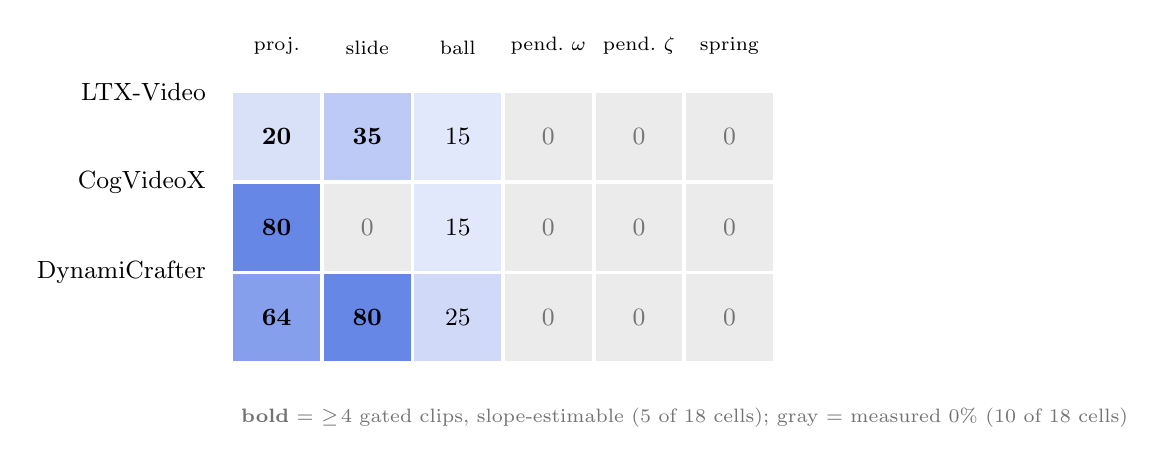
\begin{tikzpicture}[font=\small]

\def\models{{LTX-Video},{CogVideoX},{DynamiCrafter}}
\def\axes{{proj.},{slide},{ball},{pend.\ $\omega$},{pend.\ $\zeta$},{spring}}
\def\cellsize{1.15}

\foreach [count=\r from 0] \modelrow in \models {
  \node[font=\small,anchor=east] at (-0.2,{-\r*\cellsize}) {\modelrow};
}
\foreach [count=\c from 0] \axisname in \axes {
  \node[font=\scriptsize,anchor=south,align=center,rotate=0] at ({\c*\cellsize+\cellsize/2},0.35) {\axisname};
}

% Row 0: LTX-Video
\foreach [count=\c] \v/\bold in {20/1,35/1,15/0,0/0,0/0,0/0} {
  \pgfmathsetmacro{\x}{(\c-1)*\cellsize}
  \pgfmathsetmacro{\y}{0}
  \pgfmathsetmacro{\shade}{\v}
  \ifnum\bold=1
    \fill[RoyalBlue!\shade!white] (\x,-\y) rectangle ++(\cellsize,-\cellsize);
    \node[font=\small\bfseries,text=black] at ({\x+\cellsize/2},{-\y-\cellsize/2}) {\v};
  \else
    \ifnum\v=0
      \fill[black!8] (\x,-\y) rectangle ++(\cellsize,-\cellsize);
      \node[font=\small,text=black!55] at ({\x+\cellsize/2},{-\y-\cellsize/2}) {0};
    \else
      \fill[RoyalBlue!\shade!white] (\x,-\y) rectangle ++(\cellsize,-\cellsize);
      \node[font=\small,text=black] at ({\x+\cellsize/2},{-\y-\cellsize/2}) {\v};
    \fi
  \fi
  \draw[white,line width=1.4pt] (\x,-\y) rectangle ++(\cellsize,-\cellsize);
}
% Row 1: CogVideoX
\foreach [count=\c] \v/\bold in {80/1,0/0,15/0,0/0,0/0,0/0} {
  \pgfmathsetmacro{\x}{(\c-1)*\cellsize}
  \pgfmathsetmacro{\y}{\cellsize}
  \pgfmathsetmacro{\shade}{\v}
  \ifnum\bold=1
    \fill[RoyalBlue!\shade!white] (\x,-\y) rectangle ++(\cellsize,-\cellsize);
    \node[font=\small\bfseries,text=black] at ({\x+\cellsize/2},{-\y-\cellsize/2}) {\v};
  \else
    \ifnum\v=0
      \fill[black!8] (\x,-\y) rectangle ++(\cellsize,-\cellsize);
      \node[font=\small,text=black!55] at ({\x+\cellsize/2},{-\y-\cellsize/2}) {0};
    \else
      \fill[RoyalBlue!\shade!white] (\x,-\y) rectangle ++(\cellsize,-\cellsize);
      \node[font=\small,text=black] at ({\x+\cellsize/2},{-\y-\cellsize/2}) {\v};
    \fi
  \fi
  \draw[white,line width=1.4pt] (\x,-\y) rectangle ++(\cellsize,-\cellsize);
}
% Row 2: DynamiCrafter
\foreach [count=\c] \v/\bold in {64/1,80/1,25/0,0/0,0/0,0/0} {
  \pgfmathsetmacro{\x}{(\c-1)*\cellsize}
  \pgfmathsetmacro{\y}{2*\cellsize}
  \pgfmathsetmacro{\shade}{\v}
  \ifnum\bold=1
    \fill[RoyalBlue!\shade!white] (\x,-\y) rectangle ++(\cellsize,-\cellsize);
    \node[font=\small\bfseries,text=black] at ({\x+\cellsize/2},{-\y-\cellsize/2}) {\v};
  \else
    \ifnum\v=0
      \fill[black!8] (\x,-\y) rectangle ++(\cellsize,-\cellsize);
      \node[font=\small,text=black!55] at ({\x+\cellsize/2},{-\y-\cellsize/2}) {0};
    \else
      \fill[RoyalBlue!\shade!white] (\x,-\y) rectangle ++(\cellsize,-\cellsize);
      \node[font=\small,text=black] at ({\x+\cellsize/2},{-\y-\cellsize/2}) {\v};
    \fi
  \fi
  \draw[white,line width=1.4pt] (\x,-\y) rectangle ++(\cellsize,-\cellsize);
}

\node[font=\scriptsize,black!55,anchor=north west,align=left] at (0,-3.9)
  {\textbf{bold} = $\ge\!4$ gated clips, slope-estimable (5 of 18 cells);
   gray = measured $0\%$ (10 of 18 cells)};

\end{tikzpicture}
}
\caption{The coverage surface (\texttt{tab:coverage}) redrawn as a
heatmap. Candidate as a faster-to-read alternative or companion to the
text table.}
\end{figure}

\clearpage
\section{Failure taxonomy (creative summary)}
\begin{figure}[h]\centering
\resizebox{\textwidth}{!}{% fig_failure_taxonomy.tex -- creative/compact summary: the three failure
% modes actually found, one icon+label per mode, meant for a talk slide or
% as a small compact companion figure near the abstract/teaser. Draft only.

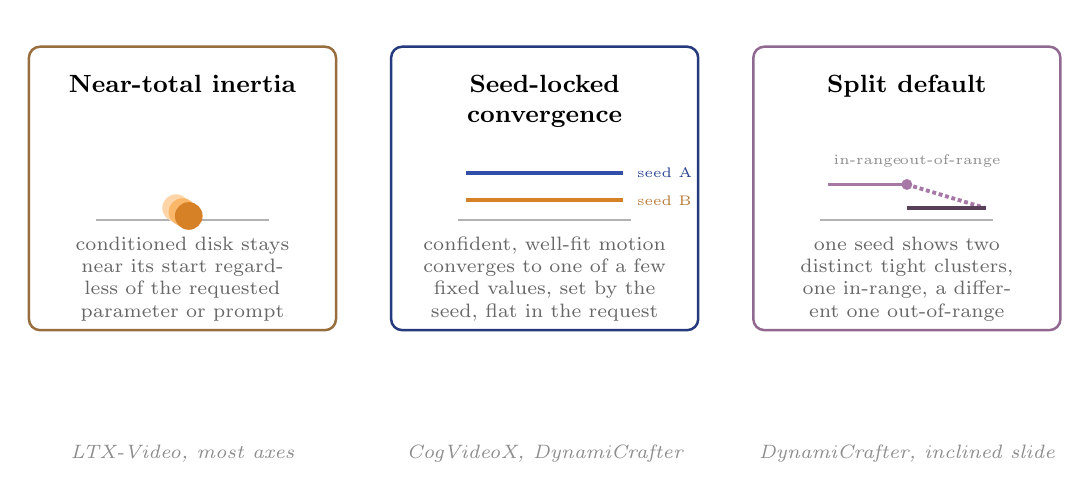
\begin{tikzpicture}[
  font=\small,
  card/.style={draw=black!25, rounded corners=4pt, minimum width=3.9cm,
               minimum height=3.6cm, fill=white, line width=0.9pt, align=center},
  ttl/.style={font=\bfseries\small, align=center},
  body/.style={font=\scriptsize, black!60, align=center}
]

% ---- Card 1: near-total inertia (LTX-Video) ----
\node[card, draw=BurntOrange!55!black] (c1) at (0,0) {};
\node[ttl] at (c1.north){\vphantom{X}};
\node[anchor=north,font=\bfseries\small,text width=3.4cm,align=center] at ([yshift=-0.25cm]c1.north)
  {Near-total inertia};
% icon: a disk that barely moves, ghost trail collapsed to almost one point
\begin{scope}[shift={($(c1)+(0,0.3)$)}]
  \draw[black!30,line width=0.8pt] (-1.1,-0.7) -- (1.1,-0.7);
  \fill[BurntOrange!30] (-0.08,-0.55) circle (5pt);
  \fill[BurntOrange!55] (0,-0.6) circle (5pt);
  \fill[BurntOrange!85!black] (0.08,-0.65) circle (5pt);
\end{scope}
\node[body,text width=3.3cm] at ([yshift=-1.15cm]c1.center)
  {conditioned disk stays near its start regardless of the requested
  parameter or prompt};
\node[font=\scriptsize\itshape,black!45] at ([yshift=-1.55cm]c1.south) {LTX-Video, most axes};

% ---- Card 2: seed-locked convergence (CogVideoX, DynamiCrafter) ----
\node[card, draw=RoyalBlue!55!black] (c2) at (4.6,0) {};
\node[anchor=north,font=\bfseries\small,text width=3.4cm,align=center] at ([yshift=-0.25cm]c2.north)
  {Seed-locked convergence};
\begin{scope}[shift={($(c2)+(0,0.3)$)}]
  \draw[black!30,line width=0.8pt] (-1.1,-0.7) -- (1.1,-0.7);
  \draw[RoyalBlue!75!black,line width=1.4pt] (-1.0,-0.1) -- (1.0,-0.1);
  \draw[BurntOrange!85!black,line width=1.4pt] (-1.0,-0.45) -- (1.0,-0.45);
  \node[font=\tiny,RoyalBlue!65!black,anchor=west] at (1.05,-0.1) {seed A};
  \node[font=\tiny,BurntOrange!70!black,anchor=west] at (1.05,-0.45) {seed B};
\end{scope}
\node[body,text width=3.3cm] at ([yshift=-1.15cm]c2.center)
  {confident, well-fit motion converges to one of a few fixed values,
  set by the seed, flat in the request};
\node[font=\scriptsize\itshape,black!45] at ([yshift=-1.55cm]c2.south) {CogVideoX, DynamiCrafter};

% ---- Card 3: split default ----
\node[card, draw=Plum!65!black] (c3) at (9.2,0) {};
\node[anchor=north,font=\bfseries\small,text width=3.4cm,align=center] at ([yshift=-0.25cm]c3.north)
  {Split default};
\begin{scope}[shift={($(c3)+(0,0.3)$)}]
  \draw[black!30,line width=0.8pt] (-1.1,-0.7) -- (1.1,-0.7);
  \draw[Plum!75!black,line width=1.4pt] (-1.0,-0.25) -- (0,-0.25);
  \draw[Plum!75!black,line width=1.4pt,densely dotted] (0,-0.25) -- (1.0,-0.55);
  \draw[Plum!40!black,line width=1.4pt] (0,-0.55) -- (1.0,-0.55);
  \node[circle,fill=Plum!75!black,inner sep=1.4pt] at (0,-0.25) {};
  \node[font=\tiny,black!45] at (-0.5,0.05) {in-range};
  \node[font=\tiny,black!45] at (0.55,0.05) {out-of-range};
\end{scope}
\node[body,text width=3.3cm] at ([yshift=-1.15cm]c3.center)
  {one seed shows two distinct tight clusters, one in-range, a different
  one out-of-range};
\node[font=\scriptsize\itshape,black!45] at ([yshift=-1.55cm]c3.south) {DynamiCrafter, inclined slide};

\end{tikzpicture}
}
\caption{The three failure modes found, as a compact icon summary.
Candidate for a talk slide or a small inset near the abstract/teaser.}
\end{figure}

\end{document}
